\chapterimage{./Images/head2.jpg} % Chapter heading image
\chapter{Course Details \& Asymptotics}
\section{Administrative Information}

\begin{itemize}
    \item Similar to ECE345, may be able to substitute lectures
    \item 5 homeworks, no extensions
    \item Textbook: CLRS (Cormen, Leiserson, Rivest, Stein)
    \item Course email: ece.algorithms+358@gmail.com
    \item Homework: 20\%
    \item \begin{itemize}
              \item Groups of 2-3
              \item You can switch Groups
          \end{itemize}
    \item Midterm: 30\%
    \item \begin{itemize}
              \item Open Textbook + Notes
          \end{itemize}
    \item Final: 45\%
    \item \begin{itemize}
              \item Open Textbook + Notes
          \end{itemize}
\end{itemize}

\section{Course Overview}
\begin{itemize}
    \item Background (Discrete Math, ~5 lectures): Asymptotic Analysis, recurrences, summations, graph/trees, permutation \& combinations
    \item Sorting (~4 lectures): Quick, Heap, Radix/Counting, Lower Bound
    \item Binary Search Trees (~3 lectures): Red-Black, searching min/max
    \item Hashing (~ 1 lecture)
    \item Greedy Algorithms (~2 lectures)
    \item Dynamic Programming (~2 lectures)
    \item \textbf{Midterm}
    \item Amoratized analysis \& splay trees (~3 lectures)
    \item Grph Algorithms (~3 lectures)
    \item \begin{itemize}
              \item Basic (~1 lecture)
              \item MSTs (~1 lecture)
              \item Shortest Paths (~1 lecture)
              \item Max Flow (~2 lecture)
          \end{itemize}
    \item History of Computations (~1 lecture)
    \item NP-Completeness (~5 lectures)
    \item Blockchain \& Cryptography (After hours)
\end{itemize}

\section{Asymptotics}
\begin{remark}
    \textit{"When we look at input sizes large enough to make relevant only the
        order of growth of the running time, we are studying the asymptotic
        efficiency of algorithms. That is, we are concerned with how the running
        time of an algorithm increases with the size of the input in the limit, as
        the size of the input increases without bound. Usually, an algorithm
        that is asymptotically more efficient is the best choice for all but very
        small inputs."}
\end{remark}
\
\begin{theorem}
    [Big-$O$ Notation, Upper Bound]
    if $f(n) = O(g(n))$ then $O(g(n))$ is the set of all $f(n)$ where $\exists$ positive constants $c$ and $n_0$ such that $0 \leq f(n) \leq c\times g(n)$ for all $n \geq n_0$ \\\\
    $O(g(n)) = \{f(n) | 0 \leq f(n) \leq c\times g(n); c, n_0 \in \mathbb{R}^+; \forall n \geq n_0 \}$ \\\\
    I.e. Big-O says the algorithm $f(n)$ \textit{grows no faster than} $g(n)$.
\end{theorem}


Essentialy, we don't care about small value, we care about the upper bound of the functions $f(n)$ and $g(n)$ as $n$ approaches infinity.

\begin{example}
    \begin{align*}
        f(n)    & = 3n + 7 \in O(n)         \\
        13n + 7 & \leq 14n, n_0 = 7, c = 14
    \end{align*}
    We can see that $f(n)$ is bounded by $O(n)$ because $f(n) \leq c\times g(n)$ for all $n \geq n_0$. \\
    You can choose any $c$ and $n_0$ that satisfies the inequality.
\end{example}

\begin{example}
    \begin{align*}
        n! = 1\times 2 \times 3 \ldots n \leq n \times n \cdots n = O(n^n) \\
    \end{align*}
\end{example}

\begin{theorem}
    [Big-$\Omega$ Notation, Lower Bound]
    if $f(n) = \Omega(h(n))$ then $\Omega(g(n))$ is the set of all $f(n)$ where $\exists$ positive constants $c$ and $n_0$ such that $0 \leq c\times h(n) \leq f(n) $ for all $n \geq n_0$ \\\\
    $\Omega(h(n)) = \{f(n) | 0 \leq c\times h(n) \leq f(n); c, n_0 \in \mathbb{R}^+; \forall n \geq n_0 \}$ \\\\
    I.e. Big-$\Omega$ says the algorithm $f(n)$ \textit{grows at least as fast as} $h(n)$.
\end{theorem}
\begin{example}
    [Arithmetic Sequence]
    \begin{align*}
        1 + & 2 + 3 + \cdots + n \geq (\frac{n}{2}) + (\frac{n}{2} + 1) + \cdots + (n) \geq \frac{n}{2}\times \frac{n}{2} \\
        =   & (c = \frac{1}{4}) - n^2 = \Omega(n^2), n_0 \geq 1
    \end{align*}
\end{example}

\begin{theorem}
    [Big-$\Theta$ Notation, Tight Bound]
    We say that $f(n) = \Theta(g(n))$ \textit{iff} $f(n) = O(g(n))$ and $f(n) = \Omega(g(n))$ \\\\
    $\Theta(g(n)) = \{f(n) | 0 \leq c_1\times g(n) \leq f(n)\leq c_2 g(n) ; c_1, c_2, n_0 \in \mathbb{R}^+; \forall n \geq n_0 \}$ \\\\
    I.e. Big-$\Theta$ says the algorithm $f(n)$ \textit{grows at the same rate as} $g(n)$ and $h(n)$.
\end{theorem}
\begin{figure}[H]
    \centering
    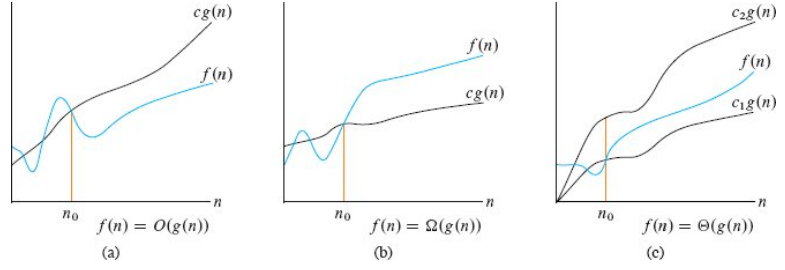
\includegraphics[scale=0.75]{./LECTURE_1/asymptotic_graphs.png}
    \caption{Asymptotic Graphs, $n_0$ is shown as the lowest possible value, but it can be any larger value}
\end{figure}
\begin{example}
    \begin{align*}
        1 + 2 + 3 + \cdots + n = \frac{n(n+1)}{2} =
        \frac{n^2}{2} + \frac{n}{2} + 1= \Theta(n^2)
    \end{align*}
\end{example}

\begin{example}
    [Summation]
    Show that $\sum_{i=1}^{n} i^k = \Theta(n^{k+1})$
    \begin{align*}
        \sum_{i=1}^{n} i^k & \leq \sum_{i=1}^{n} n^{k} = n^{k+1} = O(n^{k+1}) \\
    \end{align*}
    Therefore, $\sum_{i=1}^{n} i^k = O(n^{k+1})$, now we need to show that $\sum_{i=1}^{n} i^k = \Omega(n^{k+1})$
    \begin{align*}
        2f(n) = & \sum_{i=1}^{n}i^k + \sum_{i=1}^{n}(n-i+1)^k                 \\
        =       & 1 + 2^k + 3^k + \cdots + n^k + n^k + (n-1)^k + \cdots + 1^k \\
    \end{align*}
    \begin{align*}
        \sum_{i=1}^{n} i^k & \geq \sum_{i=\frac{n}{2}}^{n} i^k \geq \sum_{i=\frac{n}{2}}^{n} (\frac{n}{2})^k = \frac{n}{2} \times (\frac{n}{2})^k = \frac{n^{k+1}}{2^{k+1}} = \Omega(n^{k+1})
    \end{align*}
\end{example}

\subsection{Not Mentioned in Lecture, but in Assigned Reading}

\begin{definition}
    [Asymptotically Tight Bound]
    A tight bound is a bound that is as close as possible to the actual value of the function. E.g. $2n^2 = O(n^2)$ is an tight bound, but $2n = O(n^2)$ is, although correct, not asymptotically tight.
\end{definition}
\begin{theorem}
    [Little-$o$ Notation - \textbf{not} Asymptotically Tight]
    $f(n) = o(g(n))$ \textit{iff} $\forall c > 0, \exists n_0 > 0$ such that $0 \leq f(n) < c\times g(n)$ for all $n \geq n_0$
    \[o(g(n)) = \{f(n) | 0 \leq f(n) < c\times g(n); \forall c > 0; \forall n \geq n_0 \}\]
\end{theorem}

\begin{observation}
    [Big-$O$ vs Little-$o$]
    \textit{The main difference is that in $f (n) = O(g(n))$, the bound $0 \leq f (n) \leq cg(n)$ holds for some constant $c > 0$, but in $f (n) = o(g(n))$, the bound $0 \leq f (n) < cg(n)$ holds for all constants $c > 0$. Intuitively, in o-notation, the function $f (n)$ becomes insignificant relative to $g(n)$ as $n$ gets large:
        \[\lim_{n\to \infty} \frac{f(n)}{g(n)}=0\]}

\end{observation}

\begin{theorem}
    [Little-$\omega$ Notation]
    $f(n) = \omega(g(n))$ \textit{iff} $\forall c > 0, \exists n_0 > 0$ such that $0 \leq c\times g(n) < f(n)$ for all $n \geq n_0$
    \[\omega(g(n)) = \{f(n) | 0 \leq c\times g(n) < f(n); \forall c > 0; \forall n \geq n_0 \}\]
\end{theorem}

\begin{corollary}
    [The relation between $g(n)$ and $f(n) = \omega(g(n))$]
    \[\lim_{n\to \infty}\frac{f(n)}{g(n)} = \infty\]
\end{corollary}

\subsection*{Cookbook (Mentioned in Lecture)}
\begin{definition}
    [Transitivity]
    \begin{align*}
        f(n) & = \Theta(g(n)) \text{ and } g(n) = \Theta(h(n)) \implies f(n) = \Theta(h(n)), \\
        f(n) & = O(g(n)) \text{ and } g(n) = O(h(n)) \implies f(n) = O(h(n)),                \\
        f(n) & = \Omega(g(n)) \text{ and } g(n) = \Omega(h(n)) \implies f(n) = \Omega(h(n)), \\
        f(n) & = o(g(n)) \text{ and } g(n) = o(h(n)) \implies f(n) = o(h(n)),                \\
        f(n) & = \omega(g(n)) \text{ and } g(n) = \omega(h(n)) \implies f(n) = \omega(h(n)).
    \end{align*}
\end{definition}

\begin{definition}
    [Reflexivity]
    \begin{align*}
        f(n) & = \Theta(f(n)) \\
        f(n) & = O(f(n))      \\
        f(n) & = \Omega(f(n)) \\
        f(n) & = o(f(n))      \\
        f(n) & = \omega(f(n))
    \end{align*}
\end{definition}

\begin{definition}
    [Symmetry]
    \begin{align*}
        f(n) = \Theta(g(n)) \iff g(n) = \Theta(f(n))
    \end{align*}
\end{definition}

\begin{definition}
    [Transpose Symmetry]
    \begin{align*}
        f(n) = O(g(n)) \iff g(n) = \Omega(f(n)) \\
        f(n) = o(g(n)) \iff g(n) = \omega(f(n))
    \end{align*}
\end{definition}

\begin{definition}
    [Asymptotically Smaller]
    We say that $f(n)$ is asymptotically smaller than $g(n)$ if $f(n) = o(g(n))$.
\end{definition}

\begin{definition}
    [Asymptotically Larger]
    We say that $f(n)$ is asymptotically larger than $g(n)$ if $f(n) = \omega(g(n))$.
\end{definition}

\begin{theorem}
    [Other Properties]
    \begin{align*}
        n^a             & = O(n^b) \text{ \textit{iff} } a \leq b                                                    \\
        \log_a(n)       & = O(\log_b(n)) \forall a, b                                                                \\
        c^n             & = O(d^n) \text{\textit{iff}} c \leq d                                                      \\
        \text{If } f(n) & = O(g(n)) \text{ and } h(n) = O(k(n)) \text{ then } f(n) \times h(n) = O(g(n) \times k(n)) \\
        \text{If } f(n) & = O(g(n)) \text{ and } h(n) = O(k(n)) \text{ then } f(n) + h(n) = O(max\{g(n),k(n)\})      \\
    \end{align*}

\end{theorem}